
Recall that when we write $\vec x=\mat{2\\3}$, what we actually mean is $\vec x=2\xhat+3\yhat$. The numbers $2$
and $3$ are called the coordinates of the vector $\vec x$ with respect to the standard basis.  However, in general,
subspaces have many bases, and so it is possible to represent a single vector in many ways as coordinates with
respect to \emph{many} bases.

Let $\vec x=\mat{2\\3}$; let $\mathcal E=\Set{\xhat,\yhat}$ be the standard basis for $\R^2$ and let
$\mathcal B=\Set{\vec b_1,\vec b_2}$ where $\vec b_1=\mat{1\\1}$ and $\vec b_2=\mat{1\\2}$ be another
basis for $\R^2$. Now, the coordinates of $\vec x$ with respect to $\mathcal E$ are $(2,3)$, but
the coordinates of $\vec x$ with respect to $\mathcal B$ are $(1,1)$.

XXX Figure

The coordinates $(2,3)$ and $(1,1)$ represent $\vec x$ equally well, and when solving problems, we should pick the
coordinates that make our problem the easiest\footnote{ For example, maybe in one choice of coordinates, we can avoid all 
fractions in our calculations---this could be good if you're programming a computer that rounds it.}. However, now that we
are representing vectors in multiple bases, we need a way to keep track of what coordinates correspond to which basis.

\SavedDefinitionRender{RepresentationinaBasis}

\begin{example}
	Let $\mathcal E=\Set{\xhat,\yhat}$ be the standard basis for $\R^2$ and let $\mathcal B=\Set{\vec b_1,\vec b_2}$
	where $\vec b_1=\xhat+\yhat$, and $\vec b_2 =3\yhat$ be another basis for $\R^2$. Given that $\vec v=2\xhat-\yhat$, 
	find $[\vec v]_{\mathcal E}$ and $[\vec v]_{\mathcal B}$.

	Given that $\vec v=2\xhat-\yhat$, we could find 
	\[
	    [\vec v]_{\mathcal E}=\mat{2\\-1}.
	\]
	To find $[\vec v]_{\mathcal B}$, we could use a system of equations to find $\vec v$ as a linear combination of $\vec b_1$ and $\vec b_2$. That is, set 
	\[
	    \vec v = x\vec b_1 + y\vec b_2
	\]
	and substitute for $\vec b_1$ and $\vec b_2$, we see this is equivalent to finding scalars $x,y$ so that
	\[
	    2\xhat-\yhat=x\xhat+(x+3y)\yhat.
	\]
	Solve the system 
	\[
	    \sysdelim\{.
		\systeme{
			x=2,
			x+3y=-1
		},
	\]
	We have $\vec v=2\vec b_1 - \vec b_2$. That is,
	\[
	   [\vec v]_{\mathcal B}=\mat{2\\-1}. 
	\]
\end{example}

\Heading{Notation Conventions}
In light of this notation, we need to revisit some past notation. Again, we have been writing $\vec x=\mat{1\\3}$ to mean
$\vec x=2\xhat+3\yhat$. However, given the representation-in-a-basis notation, we should be writing
\[
	\vec x=\mat{2\\3}_{\mathcal E},
\]
where $\mathcal E$ is the standard basis for $\R^2$. We should write $\mat{2\\3}_{\mathcal E}$ because the coordinates $(2,3)$
refer to \emph{different} vectors for \emph{different} bases. However, most of the time we are only thinking about the standard
basis. So, the convention we will follow is:
\begin{itemize}
	\item If a problem involves only one basis, we may write $\mat{x\\y}$ to mean $\mat{x\\y}_{\mathcal E}$ where
	$\mathcal E$ is the standard basis.
	\item If there are multiple bases in a problem, we will always write $\mat{x\\y}_{\mathcal X}$ to specify a vector in
	coordinates relative to a particular basis $\mathcal X$.
\end{itemize}

\begin{emphbox}[Takeaway]
	If a problem only involves the standard basis, we may use the notation we always have. If a problem involves
	multiple bases, we must \emph{always} use representation-in-a-basis notation.
\end{emphbox}


\Heading{True Vectors vs\mbox{.} Representations}

\begin{center}
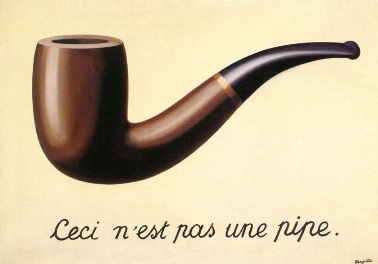
\includegraphics[width=3in]{images/MagrittePipe.jpg}\footnote{Image taken from Wikipedia: \url{https://en.wikipedia.org/wiki/File:MagrittePipe.jpg}} 
\end{center}
The Belgian surrealist Ren\'e Magritte painted the work above, which is subtitled, ``This is not a pipe''. Why? Because, of course, it is not
a pipe. It is a painting of a pipe! In this work, Magritte points out a distinction that will soon become very important to
us---the distinction between an object and a representation of that object.



Let $\vec x=2\xhat+3\yhat\in \R^2$. The vector $\vec x$ is a \emph{real-life geometrical thing}, and to
emphasize this, we will call $\vec x$ a \emph{true} vector. In contrast, when we write
the column matrix $[\vec x]_{\mathcal E}=\mat{2\\3}$, we are writing a \emph{list of numbers}. The list of
numbers $\mat{2\\3}$ has no meaning until we give it a meaning by assigning it a basis. For example,
by writing $\mat{2\\3}_{\mathcal E}$ we declare that the numbers $2$ and $3$ are coefficients of $\xhat$ and
$\yhat$. By writing $\mat{2\\3}_{\mathcal B}$ where $\mathcal B=\Set{\vec b_1,\vec b_2}$,
we declare that the numbers $2$ and $3$ are coefficients of $\vec b_1$ and $\vec b_2$. Since a list of numbers
without a basis has no meaning, we must write
\[
	\vec x\,\,{\color{Red}\neq}\,\,\, [\vec x]_{\mathcal E}=\mat{2\\3},
\]
since the left side of the equation is a \emph{true vector} and the right side is a \emph{list of numbers}. Similarly,
we must write
\[
	[\vec x]_{\mathcal E}\,\,{\color{Red}\neq}\,\,\, \mat{2\\3}_{\mathcal E}=\vec x,
\]
since the left side is a \emph{list of numbers} and the right side is a \emph{true vector}.

To help keep the notation straight in your head, for a basis $\mathcal X$, remember the rule
\[
	[\text{true vector}]_{\mathcal X} = \text{list of numbers}\qquad\text{and}\qquad
	[\text{list of numbers}]_{\mathcal X} =\text{true vector}.
\]

It's easy to get confused when answering questions that involve multiple bases; precision will
make these problems much easier.

\Heading{Orientation of a Basis}
How can you tell the difference between a hand and a foot? They're similar in structure\footnote{ We might
say hands and feet are \emph{topologically} equivalent.}---a hand has five
fingers and a foot has five toes---but they're different in shape---fingers are much longer than toes and the thumb sticks off
the hand at a different angle than the big toe sticks off the foot.

How about a harder question: how can you tell the difference between a left hand and a right hand? Any length
or angle measurement you make on an (idealized) left hand or right hand will be identical. But, we know they're different
because they differ in \emph{orientation}\footnote{ Other words for orientation include \emph{chirality} and \emph{handedness}.}.

We'll build up to the definition of orientation in stages. Consider the ordered bases $\mathcal E$, $\mathcal A$, and
$\mathcal B$ shown below.

XXX Figure

The $\mathcal A$ basis can be rotated to get the $\mathcal E$ basis, but it is impossible to rotate the $\mathcal B$ basis
to get the $\mathcal E$ basis. In this case, we say that $\mathcal E$ and $\mathcal A$ have the same orientation and
$\mathcal E$ and $\mathcal B$ have opposite orientations. In this way, even though the lengths and angles between all
vectors in the $\mathcal A$ basis and the $\mathcal B$ basis are the same, we can distinguish the $\mathcal A$ and $\mathcal B$
bases because they have different \emph{orientations}.

Orientations of bases come in exactly two flavors: \emph{right-handed} (or \emph{positively oriented})
and \emph{left-handed} (or \emph{negatively oriented}). By convention, the standard basis is called right-handed.

Orthonormal bases---bases consisting of unit vectors that are orthogonal
to each other---are called right-handed if they can be rotated to align with the standard basis, otherwise
they are called left-handed. In this way, the right-hand--left-hand analogy should be clear: two right hands or
two left hands can be rotated
to align with each other, but a left hand and a right can never be rotated to alignment.


However, not all bases are orthonormal! Consider the bases $\mathcal E$, $\mathcal A'$, $\mathcal B'$.

XXX Figure where A' and B' differ only slightly from A and B

The bases $\mathcal A'$ and $\mathcal B'$ differ only slightly from $\mathcal A$ and $\mathcal B$. Neither can
be \emph{rotated} to obtain $\mathcal E$, however we'd still like to say $\mathcal A'$ is right-handed and
$\mathcal B'$ is left-handed. The following, fully general definition, allows us to do so.

\SavedDefinitionRender{OrientationofaBasis}

The term \emph{continuously transformed} can be given a precise definition\footnote{ Because you crave precision, here it is:
the basis $\vec a_1,\ldots, \vec a_n$ can be \emph{continuously transformed} to the basis $\vec b_1,\ldots,\vec b_n$ if there
exists a continuous function $\Phi:[0,1]\to\Set{\text{$n$-tuples of vectors}}$ so that $\Phi(0)=(\vec a_1,\ldots,\vec a_n)$
and $\Phi(1)=(\vec b_1,\ldots,\vec b_n)$. Here, continuity is defined in the multi-variable calculus sense.
}, but it will be enough for us
to imagine that there is a continuous transform of one basis to another if there is a ``movie'' where one
basis smoothly and without jumps transforms into another basis.

Let's consider some examples. Let $\mathcal X=\Set{\vec x_1,\vec x_2}$. We could imagine $\vec x_1,\vec x_2$ continuously 
transforming to $\xhat, \yhat$ by $\vec x_1$ staying in place and $\vec x_2$ smoothly moving along the dotted
line.

XXX Figure

Because at every step along this motion, the set of $\vec x_1$ and the transformed $\vec x_2$ stayed linearly independent, $\mathcal X$ is
\emph{positively} oriented.

Let $\mathcal Y=\Set{\vec y_1,\vec y_2}$. We are in a similar situation, except this time, somewhere along $\vec y_2$'s path,
the set of $\vec y_1$ and the transformed $\vec y_2$ becomes linearly dependent.

XXX Figure

Maybe that was just bad luck and we might be able to transform along a different path and stay linearly independent?
It turns out, we are doomed to fail, because $\mathcal Y$ is \emph{negatively} oriented.

\bigskip

Using the definition of the orientation of a basis to answer questions is difficult because to determine
that a basis is negatively oriented, you need to make a determination about \emph{every possible} way 
to continuously transform a basis to the standard basis. This is hard enough in $\R^2$ and gets much harder
in $\R^3$. Fortunately, we will encounter computational tools that will allow us to numerically determine
the orientation of a basis, but, for now, the idea is what's important.

\Heading{Reversing Orientation}

Reflections reverse orientation and can manifest in two ways\footnote{ Think back to hands. The left
and right hands \emph{are} reflections of each other.}.
Consider the reflection of $\mathcal E=\Set{\xhat, \yhat}$ across the line $y=x$.

XXX Figure

This reflection sends $\Set{\xhat,\yhat}\mapsto\Set{\yhat,\xhat}$. Alternatively, reflection across the line $x=0$ sends
$\Set{\xhat,\yhat}\mapsto\Set{-\xhat,\yhat}$. 

XXX Figure

Both $\Set{\yhat,\xhat}$ and $\Set{-\xhat,\yhat}$, as ordered bases,
are negatively oriented. This is indicative of a general theorem.

\begin{theorem}
	Let $\mathcal B=\Set{\vec b_1,\ldots,\vec b_n}$ be an ordered basis.
	The ordered basis obtained from $\mathcal B$ by replacing $\vec b_i$ with $-\vec b_i$
	and the ordered basis obtained from $\mathcal B$ by swapping the order of $\vec b_i$ and
	$\vec b_{i+1}$ have the opposite orientation as $\mathcal B$.
\end{theorem}





